\documentclass[../ZF_Wing.tex]{subfiles}
\begin{document}

\subsection{Materialwirtschaft}
\colorbox{blue!30}{\textbf{Materialbewegung:}}
\begin{itemize}
	\item Verwaltung
	\item Planung
	\item Steuerung
	
\end{itemize}

\colorbox{blue!30}{\textbf{2 Aufgaben:}}
\begin{enumerate}
	\item Technische Aufgabe
	\item Wirtschaftliche Aufgabe

\end{enumerate}


\colorbox{blue!30}{\textbf{Bestandteile:}}
\begin{itemize}
	\item Beschaffungslogistik
	\begin{itemize}
		\item Bedarfsermittlung
		\item Beschaffungsmarktforschung
	\end{itemize}
	\item Produktionslogistik
	\begin{itemize}
		\item Verbrauchsermittlung
		\item Produktionsplanung
	\end{itemize}
	\item Lagerlogistik
	\begin{itemize}
		\item Lagerung
		\item Bestandesermittlung
	\end{itemize}
	\item Absatzlogistik
	\begin{itemize}
		\item Distribution
	\end{itemize}
	\item Entsorgungslogistik
	\begin{itemize}
		\item Entsorgung
	\end{itemize}
\end{itemize}


\begin{figure}[H]
\centering
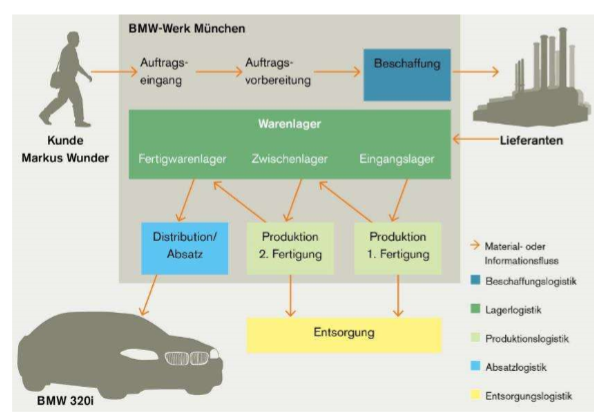
\includegraphics[width=0.3\textwidth]{Resources/Image/Logistik.png}
\caption{\label{fig:GliederungER}Logistik.}
\end{figure}


\subsubsection{Beschaffungslogistik}
\colorbox{green!30}{\textbf{Beschaffungsprozesse}}

\begin{enumerate}
	\item Ermittlung Materialbedarf für Produktion
	\item Ermittlung Lagerbestände
	\item Ermittlung Beschaffungsbedarf
	\item Lieferantenwahl
	\item Bestellungen
	\item Wareneingangskontrolle
\end{enumerate}


\colorbox{green!30}{\textbf{Beschaffungsobjekte}}
\begin{itemize}
	\item Rohstoffe
	\item Hilfsstoffe
	\item Beriebsstoffe
	\item Montageteile
	\item Handelswaren
\end{itemize}





























































































\end{document}